\documentclass[12pt]{article}

\usepackage[margin=1in]{geometry} 
\usepackage{amsmath,amsthm,amssymb}
\usepackage[spanish]{babel}
\usepackage[utf8]{inputenc}
\usepackage{tikz-cd}
\usepackage{amsmath}
\usepackage[shortlabels]{enumitem}
\usepackage{mathtools}
\usepackage{float}

\begin{document}

\title{SWAP: Ejercicio T4.2}
\author{
        Antonio Gámiz Delgado
}
\maketitle

\section{Instalación}

Vamos a instalar \textit{gobetween} en la máquina \textit{M3}, aprovechando que ya está configurada debido a la práctica 3. Por ello, primero nos aseguramos que todos los balanceadores de esa máquina están apagados:

\begin{figure}[H]
  \center
  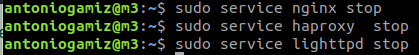
\includegraphics[scale=0.5]{img/1.png}
\end{figure}

Nos bajamos el fichero \textit{.tar.gz} de la página \cite{gobetweeninstalacion} usando \textit{curl}. Lo descomprimimos y ya está listo para usar:

\begin{figure}[H]
  \center
  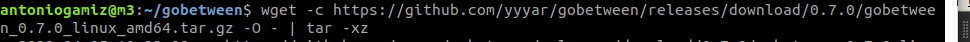
\includegraphics[scale=0.5]{img/2.png}
\end{figure}

Ahora tenemos que configurarlo como balanceador para \textit{M1} y \textit{M2}. El archivo de configuración se encuentra en \textit{config/gobetween.toml}. Lo modificamos:

\begin{figure}[H]
  \center
  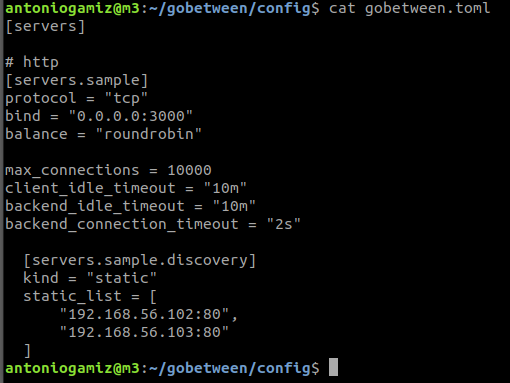
\includegraphics[scale=0.5]{img/3.png}
\end{figure}

Y lo ejecutamos:

\begin{figure}[H]
  \center
  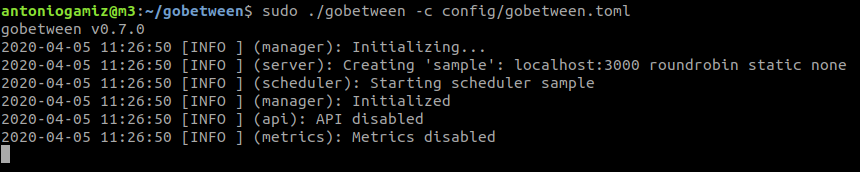
\includegraphics[scale=0.5]{img/4.png}
\end{figure}

Comprobamos que funciona correctamente:

\begin{figure}[H]
  \center
  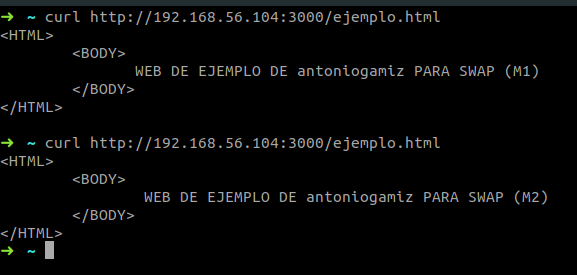
\includegraphics[scale=0.5]{img/5.png}
\end{figure}


\section{Conclusión}

Me parece que la instalación de \textit{gobetween} es más trabajosa, pero no más dificil, que los balanceadores de la práctica 3 (porque yo no uso snap). Con respecto a la configuración, me parece un poco más liosa que los dos anteriores, aunque he encontrado mucha documentación y ejemplos.

\begin{thebibliography}{9}
\bibitem{gobetween}
http://gobetween.io/
\bibitem{gobetweeninstalacion}
http://gobetween.io/downloads.html
\bibitem{balancing}
http://gobetween.io/documentation.html\#Balancing
\bibitem{docs}
http://gobetween.io/documentation.html\#Static-balancing
\bibitem{problema2}
https://github.com/yyyar/gobetween/issues/275
\end{thebibliography}
%\begin{figure}[H]
%  \center
%  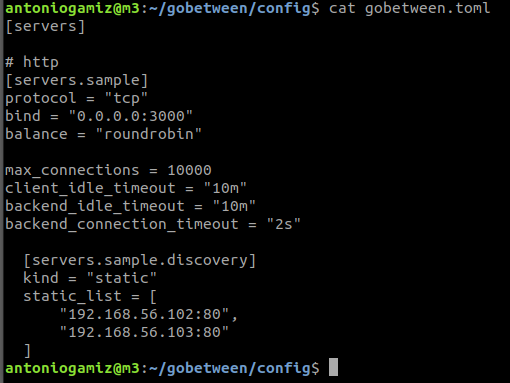
\includegraphics[scale=0.5]{img/3.png}
%\end{figure}

\end{document}
